\documentclass[russian,utf8,pointsection]{eskdtext}
\usepackage{eskdchngsheet}
\usepackage[T2A]{fontenc}
\usepackage{pscyr}
\usepackage{graphicx}
\usepackage{amstext}
\usepackage{amsmath}
\usepackage{listings}
\usepackage[unicode]{hyperref}
\usepackage{multirow}
\usepackage{listings}
\usepackage[utf8]{inputenc}
\usepackage[english,russian]{babel}

\graphicspath{{image/}}
\DeclareGraphicsExtensions{.pdf,.png,.jpg}


\ESKDdepartment{ГБОУ ВПО Нижегородский государственный технический университет им. Р. Е. Алексеева}
\ESKDcompany{Институт радиоэлектроники и информационных технологий, кафедра "Вычислительные системы и технологии"}
\ESKDtitle{Технологии распределённой обработки данных}
\ESKDdocName{Отчет к лабораторной работе №3}
\ESKDsignature{Распараллеливание алгоритма с помощью библиотеки CCR}
\ESKDauthor{Смирнова~С.~В.}
\ESKDtitleAgreedBy{Доцент каф. ВСТ}{Гай В. Е.}
\ESKDtitleDesignedBy{Студент гр. 13-В-2}{Смирнова~С.~В.}
\ESKDchecker{Гай В. Е.}
\ESKDdate{2015/12/14}

\begin{document}
	\maketitle
	\tableofcontents
	\newpage
	
	\section{Цель и порядок выполнения работы}
		  Цель работы: получить представления о возможности библиотеки Concurrent and Coordination Runtime для организации параллельных вычислений.
	
	Порядок выполнения работы:
	\begin{enumerate}
		\item Разработка последовательного алгоритма, решающего одну из приведённых задач в соответствии с выданным вариантом задания;
		\item Разработка параллельного алгоритма, соответствующий варианту последовательного алгоритма;
		\item Выполнение сравнения времени выполнения последовательного и параллельного алгоритмов обработки данных при различных размерностях исходных данных.
	\end{enumerate}
	\newpage 
	
	
	\lstset{
		breaklines=true, % Перенос длинных строк
		literate={а}{{\selectfont\char224}}1
		{б}{{\selectfont\char225}}1
		{в}{{\selectfont\char226}}1
		{г}{{\selectfont\char227}}1
		{д}{{\selectfont\char228}}1
		{е}{{\selectfont\char229}}1
		{ё}{{\"e}}1
		{ж}{{\selectfont\char230}}1
		{з}{{\selectfont\char231}}1
		{и}{{\selectfont\char232}}1
		{й}{{\selectfont\char233}}1
		{к}{{\selectfont\char234}}1
		{л}{{\selectfont\char235}}1
		{м}{{\selectfont\char236}}1
		{н}{{\selectfont\char237}}1
		{о}{{\selectfont\char238}}1
		{п}{{\selectfont\char239}}1
		{р}{{\selectfont\char240}}1
		{с}{{\selectfont\char241}}1
		{т}{{\selectfont\char242}}1
		{у}{{\selectfont\char243}}1
		{ф}{{\selectfont\char244}}1
		{х}{{\selectfont\char245}}1
		{ц}{{\selectfont\char246}}1
		{ч}{{\selectfont\char247}}1
		{ш}{{\selectfont\char248}}1
		{щ}{{\selectfont\char249}}1
		{ъ}{{\selectfont\char250}}1
		{ы}{{\selectfont\char251}}1
		{ь}{{\selectfont\char252}}1
		{э}{{\selectfont\char253}}1
		{ю}{{\selectfont\char254}}1
		{я}{{\selectfont\char255}}1
		{А}{{\selectfont\char192}}1
		{Б}{{\selectfont\char193}}1
		{В}{{\selectfont\char194}}1
		{Г}{{\selectfont\char195}}1
		{Д}{{\selectfont\char196}}1
		{Е}{{\selectfont\char197}}1
		{Ё}{{\"E}}1
		{Ж}{{\selectfont\char198}}1
		{З}{{\selectfont\char199}}1
		{И}{{\selectfont\char200}}1
		{Й}{{\selectfont\char201}}1
		{К}{{\selectfont\char202}}1
		{Л}{{\selectfont\char203}}1
		{М}{{\selectfont\char204}}1
		{Н}{{\selectfont\char205}}1
		{О}{{\selectfont\char206}}1
		{П}{{\selectfont\char207}}1
		{Р}{{\selectfont\char208}}1
		{С}{{\selectfont\char209}}1
		{Т}{{\selectfont\char210}}1
		{У}{{\selectfont\char211}}1
		{Ф}{{\selectfont\char212}}1
		{Х}{{\selectfont\char213}}1
		{Ц}{{\selectfont\char214}}1
		{Ч}{{\selectfont\char215}}1
		{Ш}{{\selectfont\char216}}1
		{Щ}{{\selectfont\char217}}1
		{Ъ}{{\selectfont\char218}}1
		{Ы}{{\selectfont\char219}}1
		{Ь}{{\selectfont\char220}}1
		{Э}{{\selectfont\char221}}1
		{Ю}{{\selectfont\char222}}1
		{Я}{{\selectfont\char223}}1
	}
	
	\lstset{
		language=Java,
		basicstyle=\footnotesize
	}
	
	
    \section{Теоретические сведения}
    \subsection{Библиотека Concurrent and Coordination Runtime}
    Библиотека Concurrent and Coordination Runtime (CCR) предназначена для организации обработки данных с помощью параллельно и асинхронно
    выполняющихся методов. Взаимодействие между такими методами организуется на основе сообщений. Рассылка сообщений основана на     использовании портов.
    Основные понятия CCR:
    \begin{enumerate}
    \item Сообщение – экземпляр любого типа данных;
    \item Порт – очередь сообщений типа FIFO (First-In-First-Out), сообщение остаётся в порте пока не будут извлечено из очереди порта     получателем.
    Определение порта:
    
    Port<int> p = new Port<int>();
    
    Отправка сообщения в порт:
    
    p.Post(1);
    
    \item получатель – структура, которая выполняет обработку сообщений.
    Данная структура объединяет:
    	\begin{itemize}
   \item один или несколько портов, в которые отправляются сообщения;
    \item метод (или методы), которые используются для обработки сообщений (такой метод называется задачей);
    \item логическое условие, определяющее ситуации, в которых активизируется тот или иной получатель.
    
    Делегат, входящий в получатель, выполнится, когда в порт intPort придёт сообщение.
    Получатели сообщений бывают двух типов: временные и постоянные (в примере получатель – временный). Временный получатель, обработав
    сообщение (или несколько сообщений), удаляется из списка получателей сообщений данного порта.
    \end{itemize}
        
    \item процессом запуска задач управляет диспетчер. После выполнения условий активации задачи (одним из условий активации может быть
    получение портом сообщения) диспетчер назначает задаче поток из пула потоков, в котором она будет выполняться.
    Описание диспетчера с двумя потоками в пуле:
    
    Dispatcher d = new Dispatcher(2, "MyPool");
    
    Описание очереди диспетчера, в которую задачи ставятся на выполнение:
    
    DispatcherQueue dq = new DispatcherQueue("MyQueue", d);
    
    \end{enumerate}
    
       \subsection{Создание проекта}
       Нужно выполнить следующие действия:
       \begin{enumerate}
       \item Установить библиотеку CCR (CCR входит в состав Microsoft Robotics Developer Studio);
       \item Создать проект консольного приложения и добавьте к проекту библиотеку Microsoft.Ccr.Core.dll.
       	\end{enumerate}
       	
       	\subsection{Оценка времени выполнения}
       	Время выполнения вычислений будем определять с помощью класса
       	\begin{lstlisting}
       	Stopwatch:       	
       	Stopwatch sWatch = new Stopwatch();       	
       	sWatch.Start();       	
       	<выполняемый код>       	
       	sWatch.Stop();       	
       	Console.WriteLine(sWatch.ElapsedMilliseconds.ToString());
       	      	\end{lstlisting}
       	
       	\section{Выполнение лабораторной работы}
       		\subsection{Вариант задания}
       		Вариант 13:
       		\begin{itemize}
       			\item Разработать алгоритм сортировки массива чисел методом пузырька
       		\end{itemize}
       	\subsection{Листинг программы}
       
     
  \lstinputlisting[language=Java]
   {Program.cs}
       	
       	\subsection{Результат работы программы}
       	Скриншот работы программы представлен на Рис.\ref{ris:1_1}. и Рис. \ref{ris:1_2}.
       	\begin{figure}[!h]
       		\centering{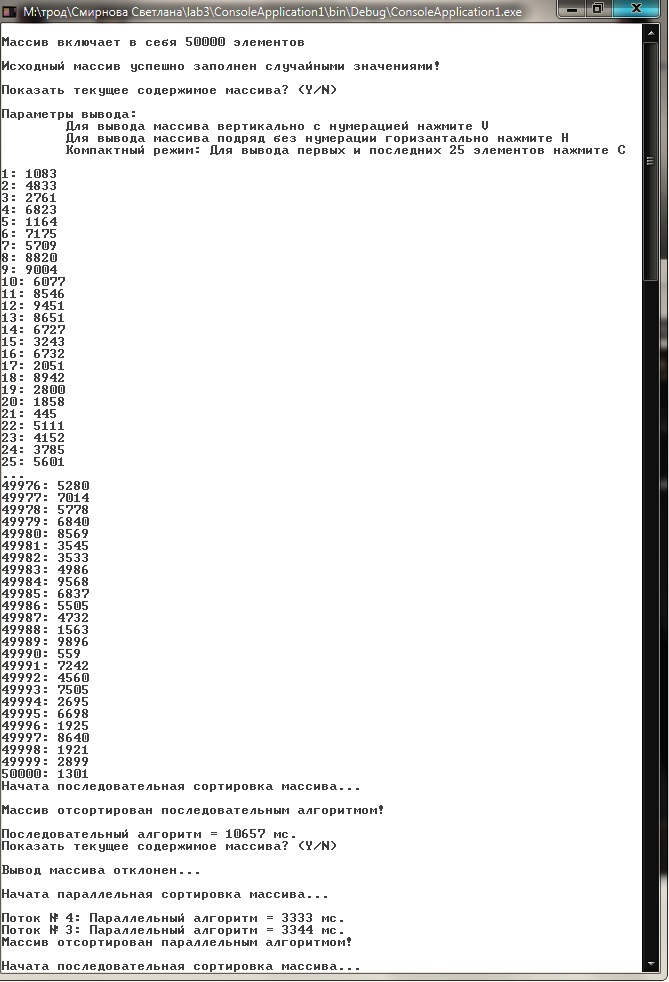
\includegraphics[scale = .4]{1_1}}
       		\caption{}
       		\label{ris:1_1}
       	\end{figure}
       	\begin{figure}[!h]
       		\centering{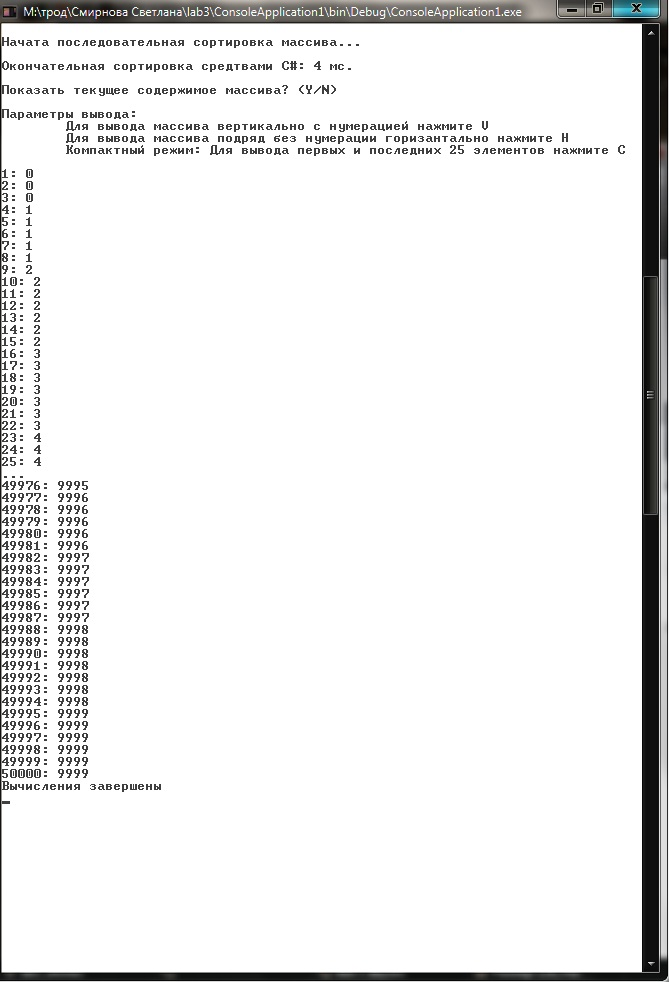
\includegraphics[scale = .4]{1_2}}
       		\caption{}
       		\label{ris:1_2}
       	\end{figure}       	

    \newpage    	   	
	\section{Вывод}
	В результате выполнения лабораторной работы мы получили представление о возможности библиотеки Concurrent and Coordination Runtime для организации параллельных вычислений.
	Мы выяснили, что скорость работы параллельного алгоритма превосходит скорость работы последовательного алгоритма. Быстродействие параллельного алгоритма напрямую зависит от числа используемых ядер.
		
\end{document}